\chapter{PELAKSANAAN PENELITIAN}
\label{pelaksanaan-penelitian}

\section{Alat dan Bahan Penelitian}
Penelitian yang dilakukan menggunakan beberapa alat dan bahan yang disebutkan pada Tabel \ref{tbl:4:alatbahan}, dan Tabel \ref{tbl:4:speklaptop}.

\vspace{0em}
\begin{table}[!h]
	\caption{Daftar alat dan bahan}
	\label{tbl:4:alatbahan}
	\centering
	% use packages: array
	\begin{tabular}{|c|p{5cm}|p{8cm}|}
		\hline
		No. & Nama alat/bahan & Fungsi \\
		\hline
		1 & Laptop ASUS N550JX & Perangkat komputer perancangan jaringan saraf tiruan. \\
		\hline
		2 & Python versi 3.7 & Bahasa pemrograman. \\
		\hline
		3 & Visual Studio Code versi 1.38 & Aplikasi penulisan dan penyuntingan kode sumber. \\
		\hline
		4 & Jupyter Notebook 1.0 & Aplikasi web untuk menulis kode program, teks, persamaan, dan visualisasi. \\
		\hline
		5 & Scikit-Learn versi 0.21 & Pustaka pembangunan jaringan saraf tiruan. \\
		\hline
		%6 & Raspberry Pi versi 3 B & Komputer mikro sebagai perangkat pengendali. \\
		%\hline
	\end{tabular}
\end{table}
\vspace{-1em}
\begin{table}[!h]
	\caption{Spesifikasi laptop ASUS N550JX}
	\label{tbl:4:speklaptop}
	\centering
	% use packages: array
	\begin{tabular}{|c|p{5cm}|p{8cm}|}
		\hline
		No. & Komponen & Spesifikasi \\ 
		\hline
		1 & Processor & Intel Core i7-4720HQ CPU @ 2.60GHz x 8 \\ 
		\hline
		2 & Graphics & Intel Haswell Mobile \\
		\hline
		3 & RAM & 8 GB \\ 
		\hline
		4 & Tipe sistem operasi & 64-bit \\
		\hline
		5 & Sistem operasi & Manjaro Linux \\ 
		\hline
	\end{tabular}
\end{table}

\section{Tata Laksana Penelitian}
Alur penelitian yang digunakan penulis dalam mencapai tujuan dapat dilihat pada Gambar \ref{fig:4:TataLaksanaPenelitian} dan Gambar \ref{fig:4:DiagramRancangBangun} berikut.
\begin{figure}[!h]
	\centering
	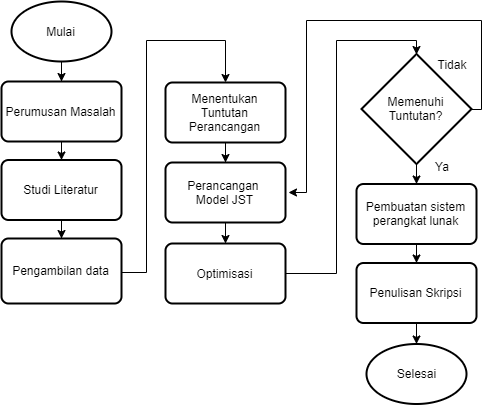
\includegraphics[width=0.7\textwidth]{figures/AlurPenelitian}
	\caption{Diagram Alir Tata Laksana Penelitian}
	\label{fig:4:TataLaksanaPenelitian}
\end{figure}
\begin{figure}[!h]
	\centering
	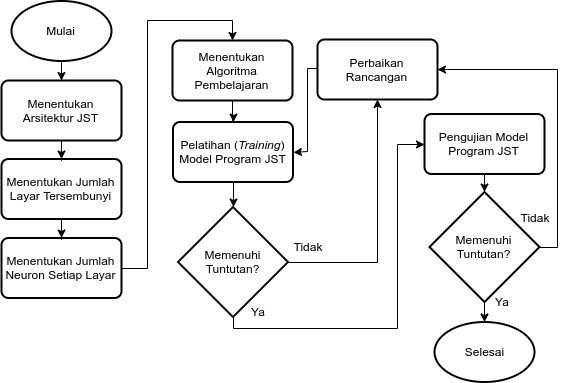
\includegraphics[width=0.8\textwidth]{figures/TataLaksanaRancangBangun}
	\caption{Diagram Alir Rancang Bangun}
	\label{fig:4:DiagramRancangBangun}
\end{figure}

\subsection{Studi Literatur}
Studi literatur bertujuan untuk mendapatkan pemahaman dalam penyelesaian masalah yang diangkat dalam penelitian ini. Studi literatur juga membantu menegaskan tujuan penelitian sehingga penulis mampu mengetahui perbedaan penelitian ini dengan penelitian terkait yang telah dilakukan sebelumnya. Dari studi literatur yang telah dilakukan maka akan memperjelas tuntutan perancangan dari sistem yang akan dibuat. Informasi yang digunakan bersumber dari berbagai artikel ilmiah, jurnal, skripsi, buku, dan/atau sumber tertulis lainnya yang membahas mengenai sistem kendali lingkungan termal dan/atau jaringan saraf tiruan.

\subsection{Pengambilan Data}
Penelitian ini menggunakan data dari model pada penelitian sebelumnya terkait karakterisasi lingkungan termal \textit{climate chamber} yang dilakukan oleh Ichfan Kurniawan. Data tersebut merupakan hasil simulasi pada \textit{software} IES-VE dengan menerapkan beberapa variasi kondisi lingkungan pada model \textit{climate chamber}.

Data yang digunakan adalah data dari model sistem di penelitian sebelumnya terkait \textbf{pemodelan lingkungan termal sistem Climate Chamber} menggunakan aplikasi IES-VE. Data yang digunakan tersusun dari beberapa variasi variabel. Variasi tersebut yaitu kondisi batas lingkungan (radiasi matahari dan suhu bola kering luar / \textit{drybulb temperature}), kondisi AC, dan kondisi \textit{heater}. Variasi kondisi batas lingkungan tersebut diwujudkan dalam pembagian 4 musim dalam 1 tahun, yakni bulan maret, juni, september dan desember. Keluaran dari model IES-VE berupa nilai suhu udara ruang (\textit{air temperature}) \textit{chamber} dan kelembapan relatif (RH) \textit{chamber}.

Data yang sudah terkumpul disajikan dalam bentuk tabular yang kemudian diolah dalam program komputer yang dibuat oleh penulis.

\subsection{Tuntutan Rancangan}

Tuntutan pada rancangan ini merujuk pada standar SNI dengan nilai standar suhu udara dijaga pada nilai 25 $\pm$ 1$^{\circ}$C dan nilai kelembapan dinyatakan dalam bentuk \textit{relative humidity} (RH), dijaga pada nilai 60\% $\pm$ 10\%. Sehingga dapat dikatakan bahwa \textit{setpoint} untuk suhu udara bernilai 25$^{\circ}$C dan untuk kelembapan udara (RH) sebesar 60\% dengan kesalahan keadaan tunak tidak melebihi 1$^{\circ}$C (suhu udara) dan 10\% (kelembapan relatif) \cite{SNI-03-06390-2000}. Nilai tersebut akan digunakan sebagai acuan untuk menganalisis perbedaan suhu udara dan kelembaban relatif antara aktual dan prediksi.

\subsection{Pemodelan Sistem Kendali}
Pada langkah ini penulis menjabarkan variabel apa saja yang terlibat dalam \textit{plant} terkait sistem kendali yang akan dibuat. Dalam suatu sistem kendali perlu diketahui variabel apa saja yang termasuk dalam kategori \textit{controlled variables}, \textit{manipulated variables}, dan \textit{disturbance variables}. \textit{Controlled variables} adalah variabel akan dikendalikan dalam suatu sistem kendali. \textit{Manipulated variables} adalah variabel yang akan mempengaruhi nilai \textit{controlled variables} melalui \textit{manipulator}/\textit{actuator}. Sementara, \textit{disturbance variables} adalah variabel yang mempengaruhi sistem tetapi perancang tidak memiliki kuasa dalam mengatur nilainya. Hasil dari identifikasi sistem
berbentuk diagram blok fungsional.

\section{Rencana Analisis Hasil Penelitian}